The process of moving an implicit surface given by a signed distance function is known as \emph{level set methods}. Level set methods are ways of influencing signed distance fields to move the implicit surfaces contained therein. This is done by solving certain equations of motion that we will describe in this section.

First we distinguish between Lagrangian and Eulerian representations of the surface.
To understand the difference between the two viewpoints we
imagine how we could measure the movement of ex. a fluid. In the Eulerian
viewpoint we would place measuring devices at fixed points in the
fluid, and continues sample the velocity of the fluid, the measured
value is taken as a avarage for an area. For convenience the
measuring devices are almost always placed in a uniform grid, with
square areas as illustrated in figure \ref{fig:eulerian}.

\begin{figure}[h]
  \centering
  \subfloat[Eulerian]{
    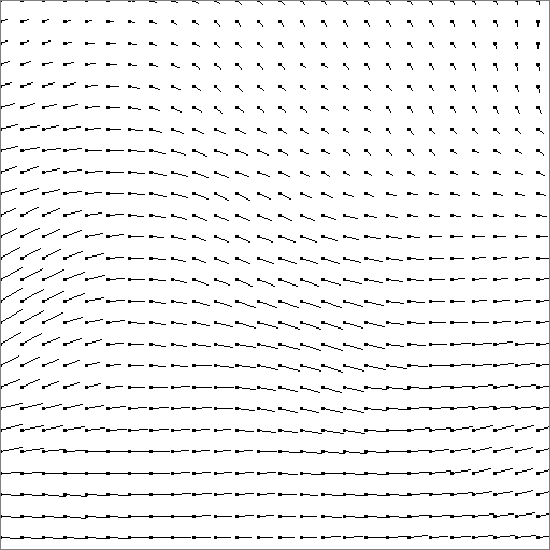
\includegraphics[width=0.5\textwidth]{imgs/eulerian.png}
    \label{fig:eulerian}
  }
  \subfloat[Lagrangian]{
    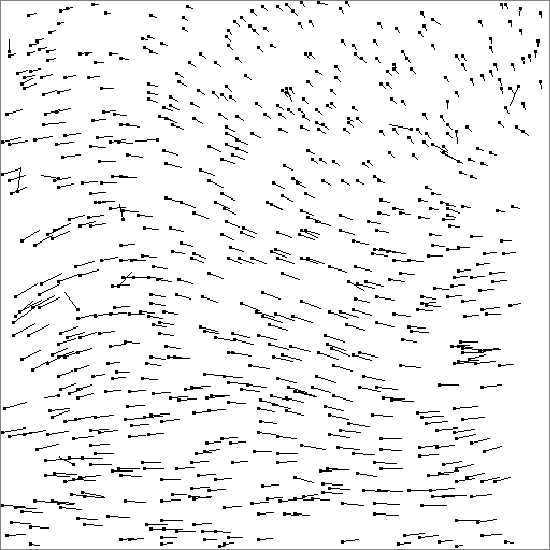
\includegraphics[width=0.5\textwidth]{imgs/lagrangian.png}
    \label{fig:lagrangian}
  }
  \caption{The eulerian and the lagrangian viewpoints.}
  \label{fig:eulerian-lagrangian}
\end{figure}

In the lagrangian viewpoint we let the measuring devices move along
the current in the fluid and take measurements at different locations
in the fluid. Here we imagine that the measuring device is part of the
fluid or a particle that the fluid moves around. Figure
\ref{fig:lagrangian} shows how the current has moved the devices as
time has progressed.

These two viewpoints are tightly coupled to the way the simulation data
is represented and visuliazed. Lets say that we are interested in
visualizing the surface of the substance.
%
The Lagrangian data is keept as points in space and moved around by
updating the position of the points. This can be visualized by
imposing that the points define a surface and rendered as geometry
ex. triangles between the points.
%
The eulerian viewpoint is seen as a 3D grid. Each cell in the grid has
a density that describes how much substance the cell contains (0-100\%).

In the Lagrangian representation, movement by a velocity field can be accomplished by solving the ordinary differential equation:
\begin{eqnarray}
\frac{d\vec{x}}{dt} = \vec{V}\left(\vec{x}\right)
\end{eqnarray}
As discussed previously, however, using implicit surfaces by an Eulerian representation rather than an explicit Lagrangian representation, such as a polygon mesh, provides certain benifits. Nowhere is this more clear than when implementing moving surfaces. Moving a surface built from triangles presents a number of problems. First and foremost, it becomes necessary to determine whether the surface starts to overlap itself and what to do if it does. Clearly this is problematic when dealing with polygons, since there is no obvious or "natural" way of merging two polygons which have overlapped.

\image{movingsurfaces.png}{0.4}{Two moving surface representations.
Top: Explicit representation, merging is a problem.
Bottom: Implicit surface by signed distance field, merging is automatic.}{velocity:movingsurfaces}

With implicit surfaces, this problem disappears, since an implicit surface is just that: implicit. If two "interior" areas of the implicit function "overlaps", it simply means that that area of the domain is in the interior of the function, and the interface will wrap around it as appropriate. See figure \vref{velocity:movingsurfaces} for an illustration of the advantage of implicit surfaces.

\subsection{The level set equation}
We examine now how to evolve an implicit surface, or interface, by affecting the underlying implicit function with an externally generated velocity field. This process of convection in an Eulerian representation is defined by equation \vref{velocity:levelseteq}
\begin{eqnarray}
\label{velocity:levelseteq}
\phi_t + \vec{V}\cdot \nabla \phi = 0
\end{eqnarray}
This partial differential equation is referred to as the \emph{level set equation} due to its central importance to level set methods. It describes the evolution of an implicit function $\phi$ by a velocity field $\vec{V}$. $\nabla \phi$, of course, is the gradient of the function. From this, we have
\begin{eqnarray}
\label{velocity:gradient}
\vec{V}\cdot\nabla\phi = u\phi_x + v\phi_y
\end{eqnarray}
Where $\phi_x$ and $\phi_y$ are the spacial derivatives in the first two
dimensions respectively and $u$ and $v$ are the two components of the
velocity vector.

Since we are essentially only interested in moving the implicit surface or interface with the velocity field, it is sufficient for the field to contain values only in a band around the interface. For simplicity of implementation, however, we assume that the field is defined across the entire domain.

For concrete implementation purposes, to evolve an implicit surface in an n-dimensional domain, the velocity field is an n-dimensional cartesian grid of n-dimensional vectors. In our two-dimensional case, that means all velocity fields are double arrays of two-value vectors.

\subsection{Upwind differencing}
How then, do we numerically solve equation \ref{velocity:levelseteq}? As we know, the implicit function is discretized into a cartesian grid of cells with $\Delta x$ representing the width and height of these cells in the theoretical continuous field. In our case this is a discretized signed distance field, each cell in the grid being of course a number representing the distance from the zero-isocountour. So too is the velocity field represented discretely with vectors, as mentioned previously.

Now, since motion takes place across time, we will need discretize our
motion across time as well. We discretize time into steps of $\Delta
t$. The n'th time step we denote $t^n$ and the state of the cartesian
grid of our signed distance field at that time as $\phi^n$. Since the
velocity also may change over time, this too is separated into
discrete steps $\vec{V}^n$.

One way of discretizing equation \ref{velocity:levelseteq} is the simple \emph{forward Euler} method. Equation \vref{velocity:forwardeuler} shows how the time-dependant term $\phi_t$ of equation \ref{velocity:levelseteq} is discretized by forward Euler. 
\begin{eqnarray}
\label{velocity:forwardeuler}
\frac{\phi^{n+1}-\phi^n}{\Delta t}+\vec{V}^n\cdot\nabla\phi^n = 0
\end{eqnarray}
This is a first-order accurate method for time discretization, which \cit{osher2002level} suggests is adequate, based on practical experience.
Expanding the gradient as in \vref{velocity:gradient} we get
\begin{eqnarray}
\label{velocity:forwardeuler}
\frac{\phi^{n+1}-\phi^n}{\Delta t}+u\phi_{x}^n + v\phi_{y}^n = 0
\end{eqnarray}
To calculate this equation, then, we must find the spatial derivatives in the x and y directions. For this we can again use a first-order difference method. However, we need to pick a direction in which to calculate the derivative. That is, do we use
\begin{eqnarray}
D^+\phi &\approx & \frac{\phi_{i+1} - \phi_i}{\Delta x} \texttt{ or}\\
D^-\phi &\approx & \frac{\phi_i - \phi_{i-1}}{\Delta x}
\end{eqnarray}
These being forward and backwards difference, respectively. Naturally, we choose by examining the velocities given for the cell in question in the velocity field and take the difference in the direction of change. Not surprisingly, the term "Upwind differencing" is derived from this way of sampling in the direction of change. 
Although it might seem natural to simply use a central difference, according to \cit{osher2002level}, this is unstable with forward Euler time discretization.

The method, then, for each cell in the grid of the implicit function is as follows:
\begin{itemize}
\item Look up the velocity in the corresponding cell in the velocity field.
\item Calculate the appropriate forward/backwards difference
\item From these, arrive at the partial spatial derivative
\item Store the new cell value
\end{itemize}
When this has been done for the entire grid, overwrite it with the new values.
Essentially, we are "collecting" the values that need to be written to the current cell of the grid in the direction they come from via the velocity grid.

To ensure stability of this method, \cit{osher2002level} recommends limiting the time-step according to the \emph{Courant-Friedrich-Lewy} condition (CFL for short) which can be written as
\begin{eqnarray}
\Delta t < \frac{\Delta x}{\max \left\lbrace \left| u \right| \right\rbrace}
\end{eqnarray}
By enforcing this, we increase the guarantee that small errors are not amplified over time. The effects of an unstable method are commonly referred to as "exploding", for obvious reasons.

Finally, \cit{osher2002level} recommends methods such as an essentially nonoscillatory (ENO) way of computing more accurate spatial differences and total variation diminishing (TVD) Runge-Kutta for further accuracy in temporal difference. In short, ENO is a polynomial forward or backward difference function and Runge-Kutta is essentially a multiple-step version of the simpler forward Euler method we use.

The above method, then, is the general solution to the problem of convecting an implicit surface by an externally generated velocity field. Using it, we may arbitrarily define our field of motion to produce motion in any way we wish.

%%% Local Variables: 
%%% mode: latex
%%% mode: auto-fill
%%% TeX-PDF-mode: t
%%% TeX-master: "../master.tex"
%%% End: 

